\documentclass[]{article}
\usepackage{vub}

\usepackage{amsmath}
\usepackage{amssymb}
\usepackage{amsthm}
\usepackage{minted}
\usepackage{graphicx}
\usepackage{subfig}
\usepackage[inkscapeformat=png]{svg}
\usepackage{parskip}

%\renewcommand{\includegraphics}{\relax}

\newcommand*{\TODO}{\textbf{TODO: }}
\newcommand*{\Gevolg}{\textbf{Gevolg: }}

\newcommand*{\so}{$\to$\ }
\newcommand*{\D}{\ensuremath{\mathcal{D}}}
\newcommand*{\T}{\ensuremath{\mathcal{T}}}
\newcommand*{\C}{\ensuremath{\mathbb{C}}}
\newcommand*{\R}{\ensuremath{\mathbb{R}}}
\newcommand*{\Q}{\ensuremath{\mathbb{Q}}}
\newcommand*{\Z}{\ensuremath{\mathbb{Z}}}
\newcommand*{\N}{\ensuremath{\mathbb{N}}}
\renewcommand*{\O}{\ensuremath{\mathcal{O}}}
\renewcommand*{\L}{\ensuremath{\mathcal{L}}}
\renewcommand*{\implies}{\ensuremath{\Longrightarrow}}
\renewcommand*{\inf}{\ensuremath{\infty}}

\renewcommand*{\boxed}[1]
{ \framebox{ \parbox[c]{0.9\textwidth}{
            #1
} } }

\title{Project VR}
\subtitle{Creating a game in OpenGL}
\author{Andreas Declerck, Sven Degelaen}

\faculty{Faculty of Science and Bio-Engineering: Computer science}

\promotors{Academic year 2022-2023}
\date{\today}

\begin{document}
\maketitle

\section{Introduction}

This document describes the implemented features in the OpenGL project for the
course VR. The assigniment is to create a game in OpenGL with as many as possible
interesting features.

\begin{figure}[h!]
      \centering
      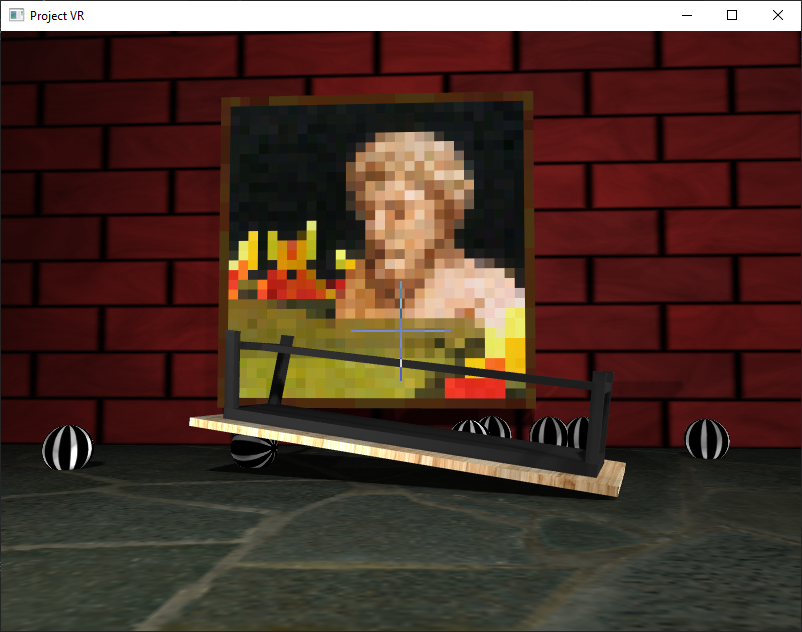
\includegraphics[width=\textwidth]{screenshot.png}
      \caption{Screenshot of the final project}
      \label{fig:screenshot}
\end{figure}

\section{Description of the game}

The game places the player in an environment where interesting effects can be
observed. This while the player's vision gets distorted to make it more
interesting.

The player is constraint to physiscs like gravity and can interact with its
environment by colliding with its surrounding objects. A mechanic was added
to make it possible to shoot little balls from the direction of where the
player is looking. Player movement can be achieved with an XBox gamepad or with
wasd + mouse. Shooting works with pressing E or on the gamepad the LB
button can be used.

Some debugging mechanics where also introduced to find more easily the
boundingboxes used for the physics. On the gamepad this is B or I on a keyboard.
Similarly a freecam option was introduced with button X on the gamepad and O on
a keyboard.
Aside from moving around, the player can jump using the spacebar, or the A button on a gamepad. 
For convenience, the window can also be put into fullscreen mode using the F11 key.

\begin{figure}[h!]
      \centering
      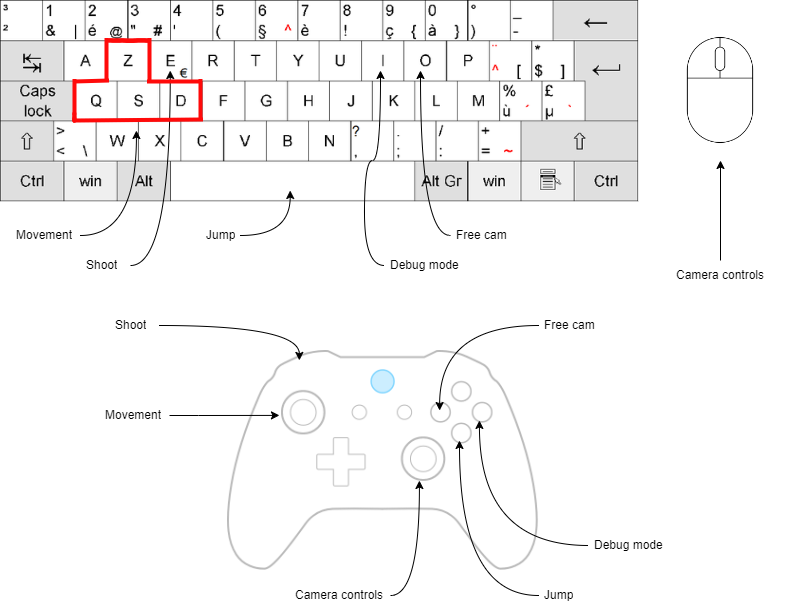
\includegraphics[width=\textwidth]{diagram.png}
      \caption{Keyboard and gamepad controls}
      \label{fig:diagram}
\end{figure}
\newpage
\section{Technical features}

To make all of this work, certain special features where introduced. These
contain:
\begin{itemize}
      \item Input processing: gamepad or keyboard + mouse implemented with glfw
      \item Automatic resizing: game screen updates when its surrounding window
            changes size (glViewport + updated framebuffer textures).
      \item Skybox: to give a sense of orientation in the scene
      \item Particle effect (moving snow whirl): based on perlin noise texture and
            created with a geometry shader which becomes periodically transparent
            (glEnable(GL\_BLEND) + fragment shader).
      \item Collision detection: bullet3 + gravity
            \begin{itemize}
                  \item Mode for viewing bounding boxes from bullet3 created with a
                        geometry shader
                  \item The camera is bound to a collision box, so the player is
                        bound to the physics in the world.
                  \item Freecam mode in which the player can detach itself from
                        collision detection boundaries.
            \end{itemize}
      \item Bullets: can be thrown and collide with other objects (fun to move
            things around with).
      \item Implemented light equations (phong shading): containing with
            attentuation and decreasing intensity with increasing distance:
            \begin{itemize}
                  \item Ambient light
                  \item Diffuse light
                  \item Specular light
            \end{itemize}
      \item Directional shadows: for both point- and spotlights with
            framebuffers where the scene is rerendered for every light with the
            possibility to exclude certain objects that do not cast a shadow.
      \item Framebuffers post-processing effect: periodically applies an edge
            detecting kernel function and adds a cross to help with aiming and uses
            inverted colors of the current frame for better visibilty of the cross.
      \item Gamma correction in a separate branch \verb|gamma_correction|.
      \item Ability to efficiently load and use external resources: by storing the
            path together with the requested resource, so duplicate calls return
            the same shared reference to the result.
      \item Ephemeral objects: Bullets can become to much in a scene and degrade
            the performance, so a system was created to remove objects if they
            fall out of the world (y < -100). Additionally a system of ephimeral
            objects was created.  These objects have a time to live (ttl) after
            which, they are destroyed.
      \item Ability to work with transparent (RGBA) and non-transparent (RGB)
            images and show them correctly
\end{itemize}

\section{Organisation of the code and external resources}

This project would not have been possible without following tools and libraries:
\begin{itemize}
      \item GLAD:\ for easy OpenGL access
      \item GLFW:\ for cross-platform access to the windowing system
      \item GLM:\ for handy linear algebra abstractions and calculations
      \item stb:\ for the easy image loading and decoding
      \item Assimp: As an abstraction for multiple 3D formats that could be
            imported into the project
      \item EnTT:\ for providing the registry in the ECS architecture used
            throughout the project
      \item Bullet3:\ for giving the structures needed to add physics to the scene
      \item CMake:\ for building the project
      \item RenderDoc:\ for debugging the rendering pipeline
\end{itemize}

The project is subdivided into 7 parts:
\begin{itemize}
      \item Shaders: resources/shaders: all the shaders used in the project
      \item Engine: src/engine: All low-level accesses to OpenGL, resource loading
            and window handling
            \begin{itemize}
                  \item The renderer has 2 buffers for the current and previous
                        frame, which are swapped when the renderer needs to send the
                        information coming from the systems to OpenGL. This done in
                        such a way that both updating and rendering are indepedent
                        except from the point where they swap contents. This to make
                        it possible (not currently implemented) to put the updating
                        proces on another thread.
                  \item All drawing calls (except some local calls in the renderer
                        itself) are protected with a RAII-guard. This gives the
                        advantage that drawing cannot be done without
                        binding/unbinding as only the guard contains the draw
                        functionality.
            \end{itemize}
      \item Scenes: src/scenes: Contains the scene of the project which bootstraps
            and updates all internal state.
      \item Components: src/components: Contains properties and higher-level
            abstractions used for implementing the game logic.
      \item Prefabs: src/prefabs: Several functions used to create entities in the
            scene and send requests to the engine to load certain resources.
      \item Systems: src/systems: The beating heart of the game part. Takes the
            entities based on their components and does calculations to advance
            the game and send the needed information to the engine. They contain
            the logic of the game.
\end{itemize}

External resources from which a lot of information was gathered on how to do
certain things in OpenGL:
\begin{itemize}
      \item Slides from course
      \item learnopengl.com
      \item docs.gl
      \item open.gl
\end{itemize}

\end{document}
